\documentclass{gescons}

\genre {Entrevista}
\author{Roberto Kunz}
\title{Seleção Consciencial - o Mecanismo Evoluído Além da Seleção Natural}


\begin{document}
    \makeentrevistatitle
    \coverart{back/Roberto_Kunz}

    \begin{multicols}{2}

\begin{center}
    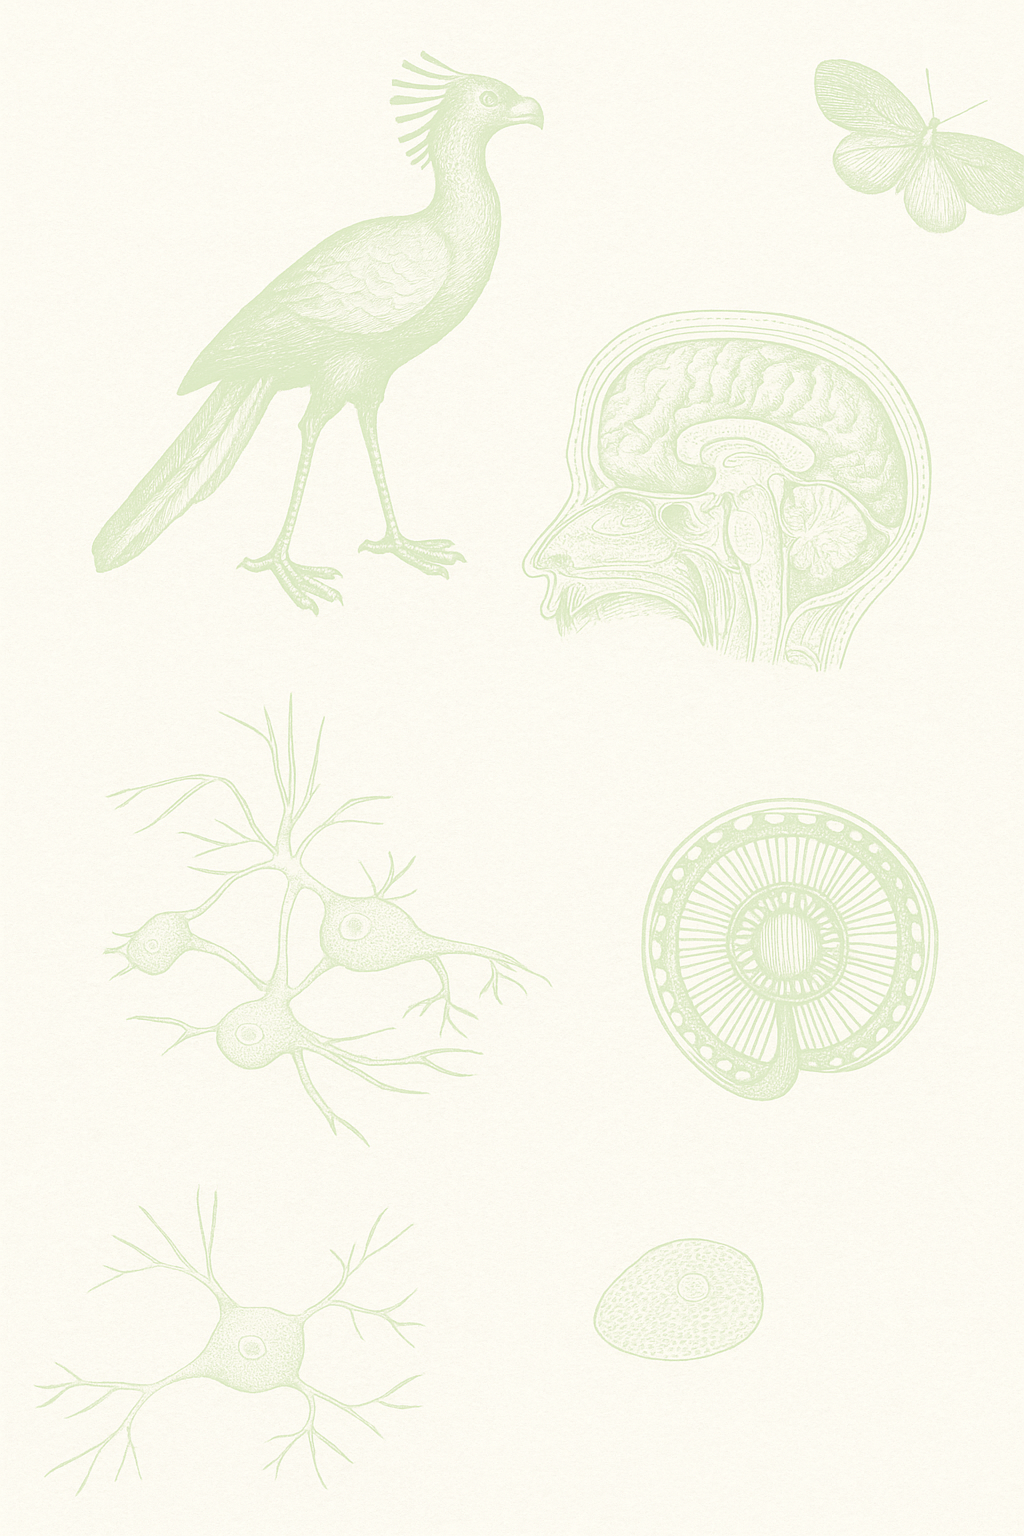
\includegraphics[width=8cm]{articles/entrevista/mockups/Roberto_Kunz.png}
\end{center}


\subsubsection{1. Qual foi a motivação para a escrita da obra? Por que a definição deste tema para publicação de um livro?}

Sempre tive o interesse em saber qual o caminho e como os animais pré-humanos chegariam à condição humana. Como essas consciências evoluem e o que poderia fazer para facilitar esta evolução. Também tenho interesse pelo estudo do comportamento animal, interesse que aumentou devido a escolha da minha profissão (Médico Veterinário). Para a escrita do livro usei como base os verbetes de minha autoria, Subumano Terapeuta, Lastro Subumano e Desanimalização Consciencial. Percebi que estes verbetes estavam interligados por um interesse em comum, então expandi esses verbetes e somei a novos estudos a respeito do tema.

\subsubsection{2. Quais foram as principais percepções, intra e extrafísicas, durante a pesquisa e a escrita da obra? E posterior ao lançamento?}

O amparo extrafísico foi constante durante a escrita do livro, a partir do momento em que criei um campo de escrita otimizado. As inspirações ficaram mais fáceis e a escrita mais fluída. Quando não tinha mais ideias, abria um livro correlato ao tema e lia no mesmo ambiente da escrita, o que possibilitava novos \emph{insights} e ideias originais a respeito do assunto. O ambiente calmo, silencioso e organizado fisicamente, possibilitou maior interação extrafísica sem dispersão. Por estar imerso nessa pesquisa e escrita, muitas vezes dormia com um problema para resolver em determinado capítulo e acordava no dia seguinte com a solução.

\begin{pullquote}
    ``As inspirações ficaram mais fáceis e a escrita mais fluída.''
\end{pullquote}

\subsubsection{3. Qual o maior aprendizado com a escrita desta obra?}


Quando comecei a escrever não tinha ideia para onde a obra caminharia, somente consegui ter a visão de conjunto após a obra concluída. Desenvolvi muitas ideias e conceitos durante a escrita, redigindo, apagando e reescrevendo até a ideia ficar clara para mim e para o leitor. Sendo assim, entendo que não é necessário saber exatamente o que vai escrever, é preciso ter um tema de interesse e pesquisar muito em livros, verbetes e artigos.


\subsubsection{4. O que poderia dizer como incentivo para que mais pesquisadores invistam na publicação de obras conscienciológicas?}

A publicação do livro permite a tares não só para o leitor mas principalmente para o escritor. As ideias se organizam e ficam mais claras para quem escreve, permitindo a especialização e aprofundamento no tema em questão. Isso permite uma assistência maior para si e para o grupo. Colocar as ideias no papel permite a conexão maior com a equipe de amparadores extrafísicos e com o público alvo da proéxis.
    
    \end{multicols}
\end{document}
